\iffalse
\documentclass[journal,12pt,twocolumn]{IEEEtran}
\usepackage{cite}
\usepackage{amsmath,amssymb,amsfonts,amsthm}
\usepackage{algorithmic}
\usepackage{graphicx}
\usepackage{textcomp}
\usepackage{xcolor}
\usepackage{txfonts}
\usepackage{listings}
\usepackage{enumitem}
\usepackage{mathtools}
\usepackage{float}
\usepackage{gensymb}
\usepackage{comment}
\usepackage[breaklinks=true]{hyperref}
\usepackage{tkz-euclide} 
\usepackage{listings}
\usepackage{gvv}                                        
\def\inputGnumericTable{}                                 
\usepackage[latin1]{inputenc}                                
\usepackage{color}                                            
\usepackage{array}                                            
\usepackage{longtable}                                       
\usepackage{calc}                                             
\usepackage{multirow}                                         
\usepackage{hhline}                                           
\usepackage{ifthen}                                           
\usepackage{lscape}
\usepackage{amsmath}
\newtheorem{theorem}{Theorem}[section]
\newtheorem{problem}{Problem}
\newtheorem{proposition}{Proposition}[section]
\newtheorem{lemma}{Lemma}[section]
\newtheorem{corollary}[theorem]{Corollary}
\newtheorem{example}{Example}[section]
\newtheorem{definition}[problem]{Definition}
\newcommand{\BEQA}{\begin{eqnarray}}
\newcommand{\EEQA}{\end{eqnarray}}
\newcommand{\define}{\stackrel{\triangle}{=}}
\theoremstyle{remark}
\newtheorem{rem}{Remark}

\usepackage{circuitikz} 

\begin{document}
{\small

\bibliographystyle{IEEEtran}
\vspace{3cm}

\title{GATE 2021 EE 47}
\author{EE23BTECH11045 - Palavelli Srija$^{*}$}

\maketitle

\bigskip

\renewcommand{\thefigure}{\theenumi}
\renewcommand{\thetable}{\theenumi}

\vspace{3cm}
\textbf{Question:} 
In the given figure, plant $G_p(s)=\frac{2.2}{(1+0.1s)(1+0.4s)(1+1.2s)}$ and compensator $G_c(s)=K\brak{\frac{1+T_1s}{1+T_2s}}$ . The external disturbance input is D(s). It is desired that when the disturbance is a unit step, the steady-state error should not exceed 0.1 unit. The minimum value of K is
\begin{figure}[h!]
    \centering
    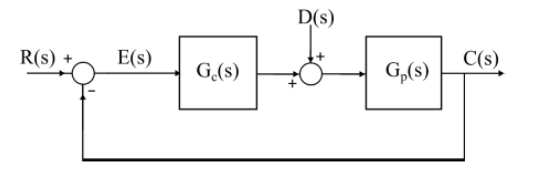
\includegraphics[width=\columnwidth]{2021/EE/47/figs/fig.png}
    \caption{}
    \label{fig:sr40}
\end{figure}
\\
\textbf{Solution:}\\
\fi
\begin{table}[h!]
    \centering
     \begin{tabular}{|c|c|}
        \hline
        \textbf{Symbol}  & \textbf{Value} \\
        \hline
        $G_p(s)$ & $\frac{2.2}{(1+0.1s)(1+0.4s)(1+1.2s)}$\\
         \hline
        $G_c(s)$& $K\brak{\frac{1+T_1s}{1+T_2s}}$  \\
         \hline
        $|e_{ss}|$& $\leq 0.1$\\
         \hline
        $K_{min}$& ??\\
        \hline
    \end{tabular}

    \caption{Input Parameters}
    \label{tab:table_omega}
\end{table}
 
\begin{align}
\text{From \figref{fig:sr40}}\notag\\
E(s) &= R(s)-C(s) \\
\text{Assume R(s)=0}\notag\\
E(s) &= -C(s) \\
C(s) &= \brak{E(s)G_c(s)+D(s)}G_p(s) \\
-E(s) &= \brak{E(s)G_c(s)+D(s)}G_p(s) \\
E(s) &= \frac{-D(s)G_p(s)}{1+G_c(s)G_p(s)} 
\end{align}
Using final value theorem 
\begin{align}
e_{ss} &= \lim_{{t \to \infty}} e(t) = \lim_{{s \to 0}} sE(s)\\
\text{Where}\quad\mathcal{L}\{e(t)\} &= E(s) \notag\\
e_{ss} &= \lim_{{s \to 0}} sE(s) \\
&= \lim_{{s \to 0}} \left(\frac{-sD(s)G_p(s)}{1+G_c(s)G_p(s)} \right) \\
\end{align}
\begin{align}
 D(s)&=\mathcal{L}\{u(t)\}  \notag\\
&=\frac{1}{s}\\
e_{ss} &=\lim_{{s \to 0}} \left(\frac{-s\frac{1}{s}G_p(s)}{1+G_c(s)G_p(s)} \right) \\
&= \lim_{{s \to 0}} \frac{\frac{-2.2}{(1+0.1s)(1+0.4s)(1+1.2s)}}{1+K\left(\frac{1+T_1s}{1+T_2s}\right)\frac{2.2}{(1+0.1s)(1+0.4s)(1+1.2s)}} \\
&= \lim_{{s \to 0}} \frac{-2.2(1+T_2s)}{(1+0.1s)(1+0.4s)(1+1.2s)(1+T_2s)+2.2K(1+T_1s)} \\
|e_{ss}| &= \frac{2.2}{1+2.2K} \\
\text{given}\notag\\ |e_{ss}|&\leq 0.1\\
\frac{2.2}{1+2.2K} &\leq 0.1 \\
K &\geq 9.54 \\
K_{\text{min}} &= 9.54
\end{align}
    %\end{document}
